\documentclass[11pt,a4paper, x11names]{article}\usepackage[]{graphicx}\usepackage[]{color}
% maxwidth is the original width if it is less than linewidth
% otherwise use linewidth (to make sure the graphics do not exceed the margin)
\makeatletter
\def\maxwidth{ %
  \ifdim\Gin@nat@width>\linewidth
    \linewidth
  \else
    \Gin@nat@width
  \fi
}
\makeatother

\definecolor{fgcolor}{rgb}{0, 0, 0}
\makeatletter
\@ifundefined{AddToHook}{}{\AddToHook{package/xcolor/after}{\definecolor{fgcolor}{rgb}{0, 0, 0}}}
\makeatother
\newcommand{\hlnum}[1]{\textcolor[rgb]{0,0,1}{\textbf{#1}}}%
\newcommand{\hlstr}[1]{\textcolor[rgb]{0.639,0.082,0.082}{#1}}%
\newcommand{\hlcom}[1]{\textcolor[rgb]{0.376,0.376,0.376}{#1}}%
\newcommand{\hlopt}[1]{\textcolor[rgb]{0,0,0}{#1}}%
\newcommand{\hlstd}[1]{\textcolor[rgb]{0,0,0}{#1}}%
\newcommand{\hlkwa}[1]{\textcolor[rgb]{0,0,1}{#1}}%
\newcommand{\hlkwb}[1]{\textcolor[rgb]{0,0,1}{#1}}%
\newcommand{\hlkwc}[1]{\textcolor[rgb]{0.169,0.569,0.686}{#1}}%
\newcommand{\hlkwd}[1]{\textcolor[rgb]{0.169,0.569,0.686}{#1}}%
\let\hlipl\hlkwb

\usepackage{framed}
\makeatletter
\newenvironment{kframe}{%
 \def\at@end@of@kframe{}%
 \ifinner\ifhmode%
  \def\at@end@of@kframe{\end{minipage}}%
  \begin{minipage}{\columnwidth}%
 \fi\fi%
 \def\FrameCommand##1{\hskip\@totalleftmargin \hskip-\fboxsep
 \colorbox{shadecolor}{##1}\hskip-\fboxsep
     % There is no \\@totalrightmargin, so:
     \hskip-\linewidth \hskip-\@totalleftmargin \hskip\columnwidth}%
 \MakeFramed {\advance\hsize-\width
   \@totalleftmargin\z@ \linewidth\hsize
   \@setminipage}}%
 {\par\unskip\endMakeFramed%
 \at@end@of@kframe}
\makeatother

\definecolor{shadecolor}{rgb}{.97, .97, .97}
\definecolor{messagecolor}{rgb}{0, 0, 0}
\definecolor{warningcolor}{rgb}{1, 0, 1}
\definecolor{errorcolor}{rgb}{1, 0, 0}
\makeatletter
\@ifundefined{AddToHook}{}{\AddToHook{package/xcolor/after}{
\definecolor{shadecolor}{rgb}{.97, .97, .97}
\definecolor{messagecolor}{rgb}{0, 0, 0}
\definecolor{warningcolor}{rgb}{1, 0, 1}
\definecolor{errorcolor}{rgb}{1, 0, 0}
}}
\makeatother
\newenvironment{knitrout}{}{} % an empty environment to be redefined in TeX

\usepackage{alltt}
\usepackage[utf8]{inputenc}
\usepackage[french]{babel}
\usepackage[left=2cm,right=2cm,top=2cm,bottom=2cm]{geometry}
\usepackage[colorlinks=true,linkcolor=black,anchorcolor=black,citecolor=black,filecolor=black,menucolor=black,runcolor=black,urlcolor=black]{hyperref} 
\usepackage[T1]{fontenc} % Font encoding
\usepackage{graphicx}
\graphicspath{{Images/}}
\usepackage{eso-pic} 
\usepackage{subfig} 
\usepackage{caption} 
\usepackage{tabu}
\usepackage{longtable}
\usepackage{transparent}
\usepackage{amsmath}
\usepackage{amsthm}
\usepackage{bm}
\usepackage{mdframed}
\usepackage[overload]{empheq}  
\usepackage{tabularx}
\usepackage{longtable}
\usepackage{colortbl}
\usepackage{cleveref}
\usepackage[square, numbers, sort&compress]{natbib} 
\bibliographystyle{plain} 
\usepackage{appendix}
\usepackage{enumitem}
\usepackage{amsthm,thmtools,xcolor} 
\usepackage{comment} % Comment part of code
\usepackage{fancyhdr} % Fancy headers and footers
\usepackage{tcolorbox} 
\usepackage{amsmath,amsfonts,amssymb}
\usepackage{pgfplots,tikz}
\usetikzlibrary{matrix}
\usepackage{enumitem}  
\usepackage[normalem]{ulem}
%fonts change 
\usepackage[charter]{mathdesign}
\usepackage{fancybox,framed}
\tcbuselibrary{skins,breakable,xparse}
\usepackage{shadowtext}
\usepackage{titlesec}
\usepackage{setspace}

\usepackage{booktabs}
\usepackage{caption}
\usepackage{float}
\usepackage{titlesec}
\usepackage{capt-of}

%dashed line
\usepackage{array}
\usepackage{arydshln}
\setlength\dashlinedash{0.2pt}
\setlength\dashlinegap{1.5pt}
\setlength\arrayrulewidth{0.3pt}

%Widows & Orphans & Penalties

\widowpenalty500
\clubpenalty500
\clubpenalty=9996
\exhyphenpenalty=50 %for line-breaking at an explicit hyphen
\brokenpenalty=4991
\predisplaypenalty=10000
\postdisplaypenalty=1549
\displaywidowpenalty=1602
\floatingpenalty = 20000
\setstretch{1.5}
\pagestyle{fancy}
\renewcommand{\footrulewidth}{0pt}
\renewcommand{\headrulewidth}{1pt}
\setlist[enumerate,1]{label=\arabic*)}
\setlength{\parindent}{0mm}
\titleformat{\section}
{\normalfont\Large\bfseries}{\thesection .}{1.5mm}{}
\titleformat{\subsection}
{\normalfont\large\bfseries}{\thesubsection}{1.5mm}{}
\titleformat{\subsubsection}
{\normalfont\normalsize\bfseries}{\thesubsubsection}{1.5mm}{}
\titleformat{\paragraph}[runin]
{\normalfont\normalsize\bfseries}{\theparagraph}{1.5mm}{}
\titleformat{\subparagraph}[runin]
{\normalfont\normalsize\bfseries}{\thesubparagraph}{1.5mm}{}

\renewcommand{\d}{\,\mathrm{d}}    

\renewcommand{\title}{Certificat de spécialisation analyste de données massives}
% -> author name and surname
\newcommand{\authora}{Boukary OUEDRAOGO}
\newcommand{\authorb}{Bangaly CAMARA}
\newcommand{\authorc}{Imad EL HAMMA}
% -> MSc course
\newcommand{\course}{STA211}
\newcommand{\advisor}{Mme Niang}
% IF AND ONLY IF you need to modify the co-supervisors you also have to modify the file Configuration_files/title_page.tex (ONLY where it is marked)
\newcommand{\firstcoadvisor}{Name Surname} % insert if any otherwise comment
\newcommand{\secondcoadvisor}{Name Surname} % insert if any otherwise comment
% -> author ID
\newcommand{\ID}{Student ID}
% -> academic year
\newcommand{\YEAR}{2021-2022}
\definecolor{bluePoli}{rgb}{0.87, 0.36, 0.51}
\definecolor{babyblueeyes}{rgb}{0.63, 0.79, 0.95}
\definecolor{blush}{rgb}{0.87, 0.36, 0.51}
\definecolor{bubblegum}{rgb}{0.99, 0.76, 0.8}
\definecolor{charcoal}{rgb}{0.21, 0.27, 0.31}
% Custom theorem environments
\declaretheoremstyle[
  headfont=\color{bluePoli}\normalfont\bfseries,
  bodyfont=\color{black}\normalfont\itshape,
]{colored}

\captionsetup[figure]{labelfont={color=charcoal}} % Set colour of the captions
\captionsetup[table]{labelfont={color=charcoal}} % Set colour of the captions
\captionsetup[algorithm]{labelfont={color=charcoal}} % Set colour of the captions

\theoremstyle{colored}
\newtheorem{theorem}{Theorem}[section]
\newtheorem{proposition}{Proposition}[section]

% Enhances the features of the standard "table" and "tabular" environments.
\newcommand\T{\rule{0pt}{2.6ex}}
\newcommand\B{\rule[-1.2ex]{0pt}{0pt}}

% Algorithm description
\newcounter{algsubstate}
\renewcommand{\thealgsubstate}{\alph{algsubstate}}
\newenvironment{algsubstates}{
  \setcounter{algsubstate}{0}%
  \renewcommand{\STATE}{%
    \stepcounter{algsubstate}%
    \Statex {\small\thealgsubstate:}\space}
}{}

% Custom theorem environment
\newcolumntype{L}[1]{>{\raggedright\let\newline\\\arraybackslash\hspace{0pt}}m{#1}}
  \newcolumntype{C}[1]{>{\centering\let\newline\\\arraybackslash\hspace{0pt}}m{#1}}
    \newcolumntype{R}[1]{>{\raggedleft\let\newline\\\arraybackslash\hspace{0pt}}m{#1}}
      
      % Custom itemize environment
      \setlist[itemize,1]{label=$\bullet$}
      \setlist[itemize,2]{label=$\circ$}
      \setlist[itemize,3]{label=$-$}
      \setlist{nosep}
      
      % Create command for background pic
      \newcommand\BackgroundPic{% Adding background picture
        \put(237,365){
          \parbox[b][\paperheight]{\paperwidth}{%
            \vfill
            \centering
            \transparent{0.4}
            \includegraphics[width=0.44\paperwidth]{raggiera_polimi.eps}%
            \vfill}
        }
      }
      
      % Set indentation
      \setlength\parindent{0pt}
      
      % Custom title commands
      \titleformat{\section}
      {\color{charcoal}\normalfont\Large\bfseries}
      {\color{charcoal}\thesection.}{1em}{}
      \titlespacing*{\section}
      {0pt}{3.3ex}{3.3ex}
      
      \titleformat{\subsection}
      {\color{charcoal}\normalfont\large\bfseries}
      {\color{charcoal}\thesubsection.}{1em}{}
      \titlespacing*{\subsection}
      {0pt}{3.3ex}{3.3ex}
      
      % Custom headers and footers
      \pagestyle{fancy}
      \fancyhf{}
      
      \fancyfoot{}
      \fancyfoot[C]{\thepage} % page
      \renewcommand{\headrulewidth}{0mm} % headrule width
      \renewcommand{\footrulewidth}{0mm} % footrule width
      
      \makeatletter
      \patchcmd{\headrule}{\hrule}{\color{black}\hrule}{}{} % headrule
      \patchcmd{\footrule}{\hrule}{\color{black}\hrule}{}{} % footrule
      \makeatother
\IfFileExists{upquote.sty}{\usepackage{upquote}}{}
\begin{document}
\begin{titlepage}
\thispagestyle{empty}

\begin{tikzpicture}[remember picture,overlay]
\node at (current page.south west)
{\begin{tikzpicture}[remember picture, overlay]
  \shade[bottom color=bubblegum,top color=white] (0,0) rectangle
  (\paperwidth,.7\paperheight);
  \node [color=gray!50,rotate=-20]at (0.35\textwidth,9){\resizebox{7cm}{1.5cm}{$\displaystyle u(x)\approx U_h=\sum_{j=1}^{N}c_j\varphi_j(x)$}};
  \node [color=gray!50,rotate=-5]at (.8\textwidth,5){\resizebox{9cm}{1.5cm}{$ \displaystyle u''(x_i ) \approx\dfrac{1}{h^2}\left[u(x_{ i+1} ) - 2u(x_i ) + u(x_{i-1 } )\right] $}
  };
  \end{tikzpicture}
};

\end{tikzpicture}
\vspace{-1cm}
%-----------------------------------------------------------------------------------
  %  page de garde
%-----------------------------------------------------------------------------------
  \begin{center}

\begin{large}

\includegraphics[scale=0.5]{Images/logocnam.png} \\
\textsc{Certificat de spécialisation analyste de données massives}\\ \bigskip
\textbf{ Entreposage et fouille de données
} \end{large}
\end{center}
\bigskip
\shadowoffset{3pt}
\begin{tcolorbox}[blanker,top=1.2cm,bottom=1.2cm,borderline horizontal={4pt}{0pt}{charcoal},colupper=bluePoli]
\begin{center}
\shadowtext{\resizebox{\textwidth}{1.5cm}{\textbf{Projet de STA211} }}
\end{center}
\end{tcolorbox}


\bigskip

\begin{minipage}{0.4\textwidth}
\large
\emph{Auteurs:}\\
\authora\\[3mm]
\authorb\\[3mm]
\authorc\\[3mm]
\end{minipage}
\hfill
\begin{minipage}{0.4\textwidth}
 \large
\emph{Professeur:}\\
\advisor\\[3mm]
\\[3mm]
\\[3mm]
\end{minipage}\\[2cm] 


\textcolor{charcoal}{\rule{.82\textwidth}{4pt}\hfill {\fontfamily{pzc}\fontsize{.7cm}{0cm}\selectfont \YEAR }}
\end{titlepage}
\tableofcontents
\begin{abstract}
\end{abstract}
\section{Introduction}
Le jeu de données CNIL est issu d'une étude menée par L'Observatoire de la Qualité de l'Air Intérieur (OQAI). L'étude a été menée sur un échantillon de 567 ménages suivis sur trois années. Les données ont été collecté en fonctions de trois grands ensembles décrivant les caractéristiques des logements, les habitudes des ménages et la composition des ménages. L'objectif de l'étude est de mesurer la qualité de l'air à l'intérieur des logements. Elle dépend de la présence de nombreux polluants physiques, biologique ou chimiques dont le formaldéhyde. Ce dernier est un polluant atmosphérique omniprésent dans les logements et dont le suivi est considéré comme étant hautement prioritaire par les pouvoirs publics depuis 2006. \par
Le but de notre de projet est d'expliquer et de prédire le formaldéhyde à partir des caractéristiques des trois ensembles de bloc de variables cités plus haut à savoir : les habitudes des ménages, les caractéristiques des ménages et la composition des ménages. Pour ce faire, nous allons nous appuyer sur différentes méthodes de datamining.
Afin de structurer notre travail, nous le scindons en deux parties. La première correspond à une exploration de données qui est préalable à tout travail de datamining. Cette étape consiste à analyser le jeu de données en unidimensionnel, en bidimensionnel et en multidimensionnel. Dans la seconde partie nous allons utiliser une méthode d'apprentissage supervisé pour modéliser et prédire le formaldéhyde.
%--------------------------------------------------------------------------------------------------
%             00-  MISE EN PLACE DE L'ENVIRONNEMENT SWEAVE POUR LA GENERATION DU DOCUMENT PDF
%--------------------------------------------------------------------------------------------------


%--------------------------------------------------------------------------------------------------
%                   01- CHARGEMENT DES PACKAGES R UTILES POUR LE TRAVAIL
%--------------------------------------------------------------------------------------------------

%--------------------------------------------------------------------------------------------------
% IMPORTATION DE LA BASE DE DONNEES ET CREATION DE SOUS BASES DE TRAVAIL
%--------------------------------------------------------------------------------------------------


%--------------------------------------------------------------------------------------------------
%                     01- SECTION : Analyse exploratoire
%--------------------------------------------------------------------------------------------------
\section{Analyse exploratoire }
Cette partie sera consacrée à l'analyse exploratoire des données.
Certaines variables qui sont codées comme des variables numériques mais qui en réalité sont qualitatives seront recordées en variables facteurs.\par
Les blocs logement et habitude sont composés respectivement de 70 variables (dont 32 variables quantitatives et 38 variables qualitatives) et 44 variables (dont 21 variables quantitatives et 23 variables qualitatives). Les caractéristiques des logements sont composées entre autres du type de logement, du type de système de ventilation, d'une information d'existence de garages attenants et des installations utilisées. Les habitudes des ménages sont décrites à travers les tâches quotidiennes des ménages notamment les tâches ménagères, la possession d'animaux de compagnie, l'utilisation de parfum et d'insecticide, etc. Le bloc ménage quant à lui contient 11 variables dont 5 variables quantitatives et 6 variables qualitatives. Ces variables décrivent la composition et la catégorie socioprofessionnelle des ménages interrogés. \par
Par ailleurs, nous avons supprimé de l'analyse deux variables qualitatives KVN2e12 et KVNT2e112 du bloc logement car elles n'ont pas de variabilité due à l'existence d'une seule modalité.\par
Pour la suite de cette partie, nous allons uniquement présenter les résultats de l'analyse exploratoire du bloc ménage. Celle des autres blocs sont présentés dans l'annexe.

% 1.1 Analayse univariée
\subsection{Analyse univariée}
Nous commençons par une analyse univariée car elle permet de résumer l'information contenu dans les variables. Elle permet également de connaître la structure, la distribution des données et de détecter les outliers. 
L'analyse univariée montre que l'âge des ménages varie entre 18 et 89 ans, avec une moyenne de 61 ans. Ils disposent d'un revenu variant entre 535 et 7600 euros avec un revenu moyen de 2574 euros. Toutefois 50\% des ménages touchent un revenu inférieur à 2349 euros et 45\% ont un revenu inférieur à 1799 euro (voir tableau \ref{tab:tab1}).
\begin{table*}[H] \centering
%\ra{1.3}
\begin{small}
\begin{tabular}{@{}lrrrrrr@{}}\toprule
\textbf{Variables}& \textbf{Moyenne} & \textbf{Médiane}& \textbf{Min} & \textbf{Maximum} & \textbf{Variance} & \textbf{Ecart-type} \\ \midrule
\textbf{Age}          & 51.87 &  52 & 18 & 89 & 209.91 & 14.49\ \\ \hdashline
\textbf{Revenus}      & 2~573.20 & 2~349 & 535&7~600 & 1~967~644.23&1~402.73   \\ \hdashline
\textbf{Nombre d'enfants dont âge > 10 ans} &  0.44 & 0 & 0 & 3 & 0.67 & 0.82  \\  \hdashline
\textbf{Nombre d'enfants dont âge <= 10 ans} &  0.32 & 0 & 0 & 3 & 0.48 & 0.70 \\
\textbf{Nombre de personnes} &  2.47 & 2 & 1 & 8 & 2.005& 1.416 \\
\bottomrule
\end{tabular}
\end{small}
\caption{Statistiques descriptives des variables quantitatives du bloc ménage}\label{tab:tab1}
\end{table*}
Les femmes représentent environ 65\% des personnes interrogées dont 50\% ont un niveau de l'enseignement technique court et seulement 30\% ont un diplôme de l'enseignement supérieur bac +2. Nous constatons la même structure chez les hommes. La principale source de revenus est le salaire et la pension avec respectivement 53\% et 34\% des sources de revenus possibles. Ils sont pour la plupart des cadres supérieurs travaillant dans des professions intermédiaires (24\%) et des ouvriers (20\%) (graphique \ref{fig1:tri_plat})
\begin{figure}[H]
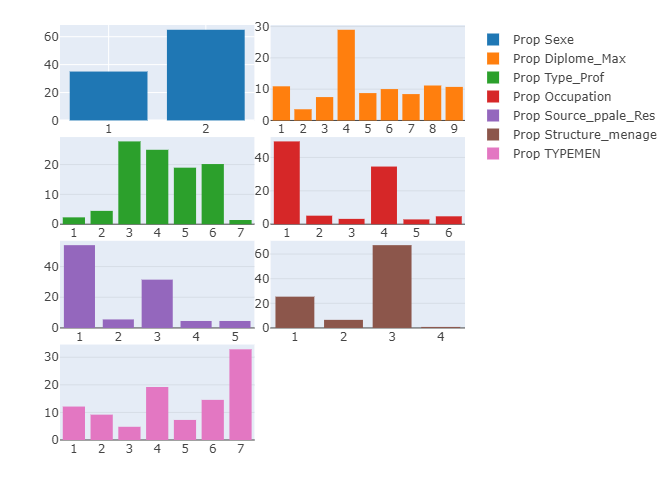
\includegraphics[scale=0.7]{graphiques/tri_plat.png}
\caption{Tri à plat des varaibles qualitatives du bloc ménage} \label{fig1:tri_plat}
\end{figure}
Cette analyse univariée nous a permis de s'apercevoir que les variables quantitatives ne sont pas à la même échelle. Nous constatons également que certaines modalités des variables qualitatives sont dominantes comme les cadres supérieurs. Cependant, c'est une analyse préalable qui faudrait approfondir via une analyse bivariée.

% 1.2
\subsection{Analyse bivariée}
L'analyse de la matrice de corrélation des variables quantitatives du bloc ménage montre, globalement, une relation faible entre les variables à l'exception le nombre de personnes composant le ménage et le nombre d'enfant quel que soit l'âge(matrice de corrélation \ref{fig2:cor})
\begin{figure}[H]
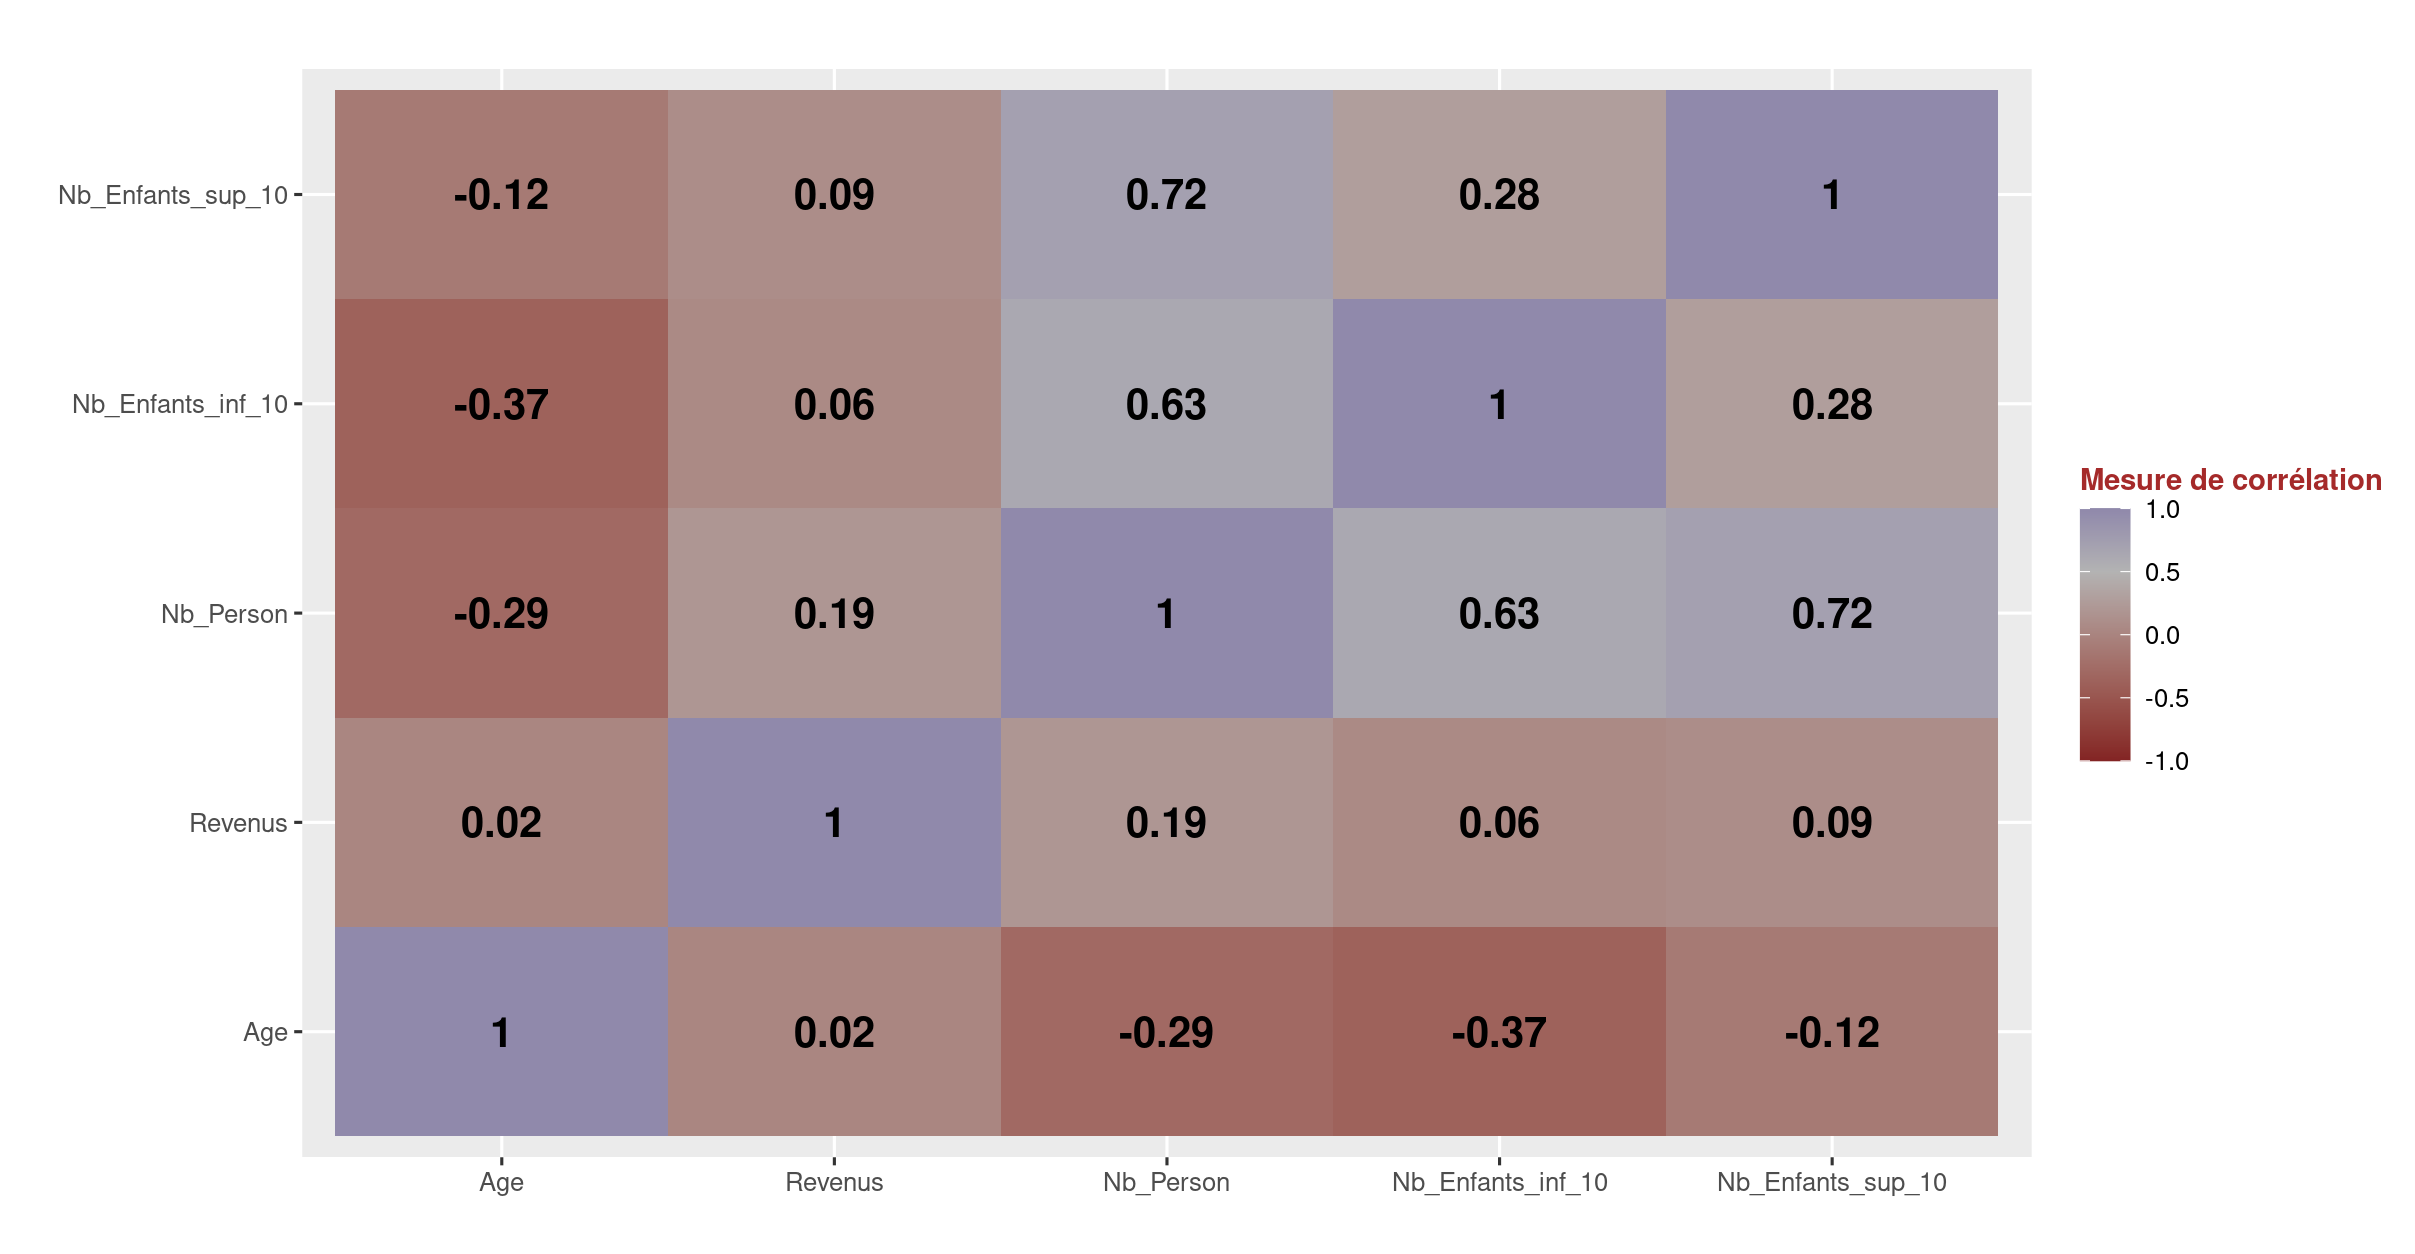
\includegraphics[scale=.6]{graphiques/corrplot.png}
\caption{Matrice des corrélations des variables qualitatives du bloc ménage} \label{fig2:cor}
\end{figure}
L'analyse du $Chi2$ de contingence et le $V$ de Cramer permet de conclure qu'il existe une relation de dépendance entre les variables quantitatives. Toutefois, celle-ci est faible à l'exception de la relation entre la source principale de revenu et l'occupation. (tableau résultat V de cramer \ref{tab2:cramer}).\par
\begin{table}[H]
\resizebox{\textwidth}{!}{%
\begin{tabular}{@{}lllllll@{}}
\toprule
                   & sexe   & type\_prof & diplome\_max & occupation & source\_ppale\_res & structure\_menage \\ \midrule
sexe               & 1      &            &              &            &                    &                   \\
type\_prof         & 0.1634 & 1          &              &            &                    &                   \\
diplome\_max       & 0.1146 & 0.1435     & 1            &            &                    &                   \\
occupation         & 0.2677 & 0.2370     & 0.1033       & 1          &                    &                   \\
source\_ppale\_res & 0.1347 & 0.1824     & 0.1091       & 0.5634     & 1                  &                   \\
structure\_menage  & 0.3495 & 0.0957     & 0.0750       & 0.1493     & 0.1866             & 1                 \\ \bottomrule
\end{tabular}%
}
\caption{Matrice des V de Cramer}
\label{tab2:cramer}
\end{table}

Après avoir terminé l'analyse bidimensionnelle dans laquelle nous n'avons pas trouvé de relation forte entre les différentes variables prises deux à deux, nous passons à l'analyse multidimensionnelle.

\subsection{Analyse exploration multidimensionnelle}
Dans l'analyse multidimensionnelle, nous avons réalisé une ACP pour les variables quantitatives, une ACM pour les variables qualitatives et une AFM pour les variables mixtes (quantitatives et qualitatives prises ensemble)
\subsubsection{Analyse en composante principale(ACP)}
Les résultats de l'ACP sur les données quantitatives des ménages montrent que le premier plan factoriel exprime plus de 67\% de la variabilité. La projection des cinq variables sur les deux premiers axes factoriels montre que le nombre d'enfant (quel que soit leur âge) et le nombre de personnes vivant dans le même foyer sont positivement corrélés à la première composante principale. Le revenu et l'âge sont fortement corrélés à la deuxième composante. Ainsi, deux structures se dégagent. La première structure est composée de l'âge et le revenu. La deuxième structure est formée par les variables nombre de personnes du foyer et le nombre d'enfants inférieur ou supérieur à 10 ans. 
La projection des individus sur le premier plan factoriel permet de distinguer quatre groupes de ménages :
\begin{itemize}
\item des ménages aisés, relativement vieux avec peu de personnes vivant sur le même toit ;
\item des ménages aisés vivant avec plusieurs personnes sur le même toit avec ou sans enfants 
\item des ménages très jeune, avec des revenus modeste et peu de personnes vivant sur le même toit. 
\end{itemize}
\begin{mdframed}
\begin{minipage}{0.45\textwidth}
\begin{figure}[H]
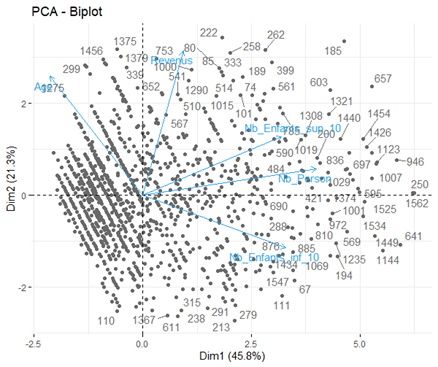
\includegraphics[]{graphiques/ACP1.png}
\caption{Graphique individus/variables de l'ACP} \label{fig3:ACP1}
\end{figure}
\end{minipage}
\hfill
\begin{minipage}{0.45\textwidth}
\begin{figure}[H]
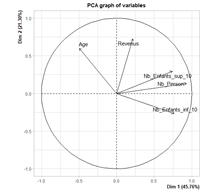
\includegraphics[]{graphiques/ACP2.png}
\caption{Cercle de corrélation} \label{fig4:ACP2}
\end{figure}
\end{minipage}
\end{mdframed}

\subsubsection{Analyse des correspondances multiples(ACM)}
Les résultats de l'ACM montrent que la première et deuxième dimension captent environ 15\% de la variabilité. Les deux catégories « occupation et source principale de ressources » sont fortement corrélées (> 0.70) avec les deux dimensions.  En revanche, les catégories « type de profession », « sexe », « structure de ménage » et le « diplôme le plus élevé » sont faiblement corrélées avec les deux axes.
La projection des variables qualitatives les plus contributives sur les deux axes montre que :
Les personnes déclarant recevoir une pension déclarent la retraite comme principale occupation.
Les étudiants déclarent autres revenus comme source principale
Les personnes déclarant avoir une activité professionnelle déclarent le salaire comme étant une source principale source de revenu.
Et enfin, si on regarde l'allure générale du nuage des individus, c'est-à-dire les ménages, on voit qu'elle est particulière et met en évidence quatre classes de ménages bien distinctes. La première bissectrice oppose les individus qui exercent une fonction (salariés) aux étudiants et ceux qui reçoivent un salaire à ceux dont le revenu provient d'un actif financier ou autres. Quant à elle, la deuxième bissectrice oppose ceux ont un diplôme de « fin études primaire » et ceux en «fin du second cycle enseignement général ».
 
\begin{mdframed}
\begin{minipage}{0.45\textwidth}
\begin{figure}[H]
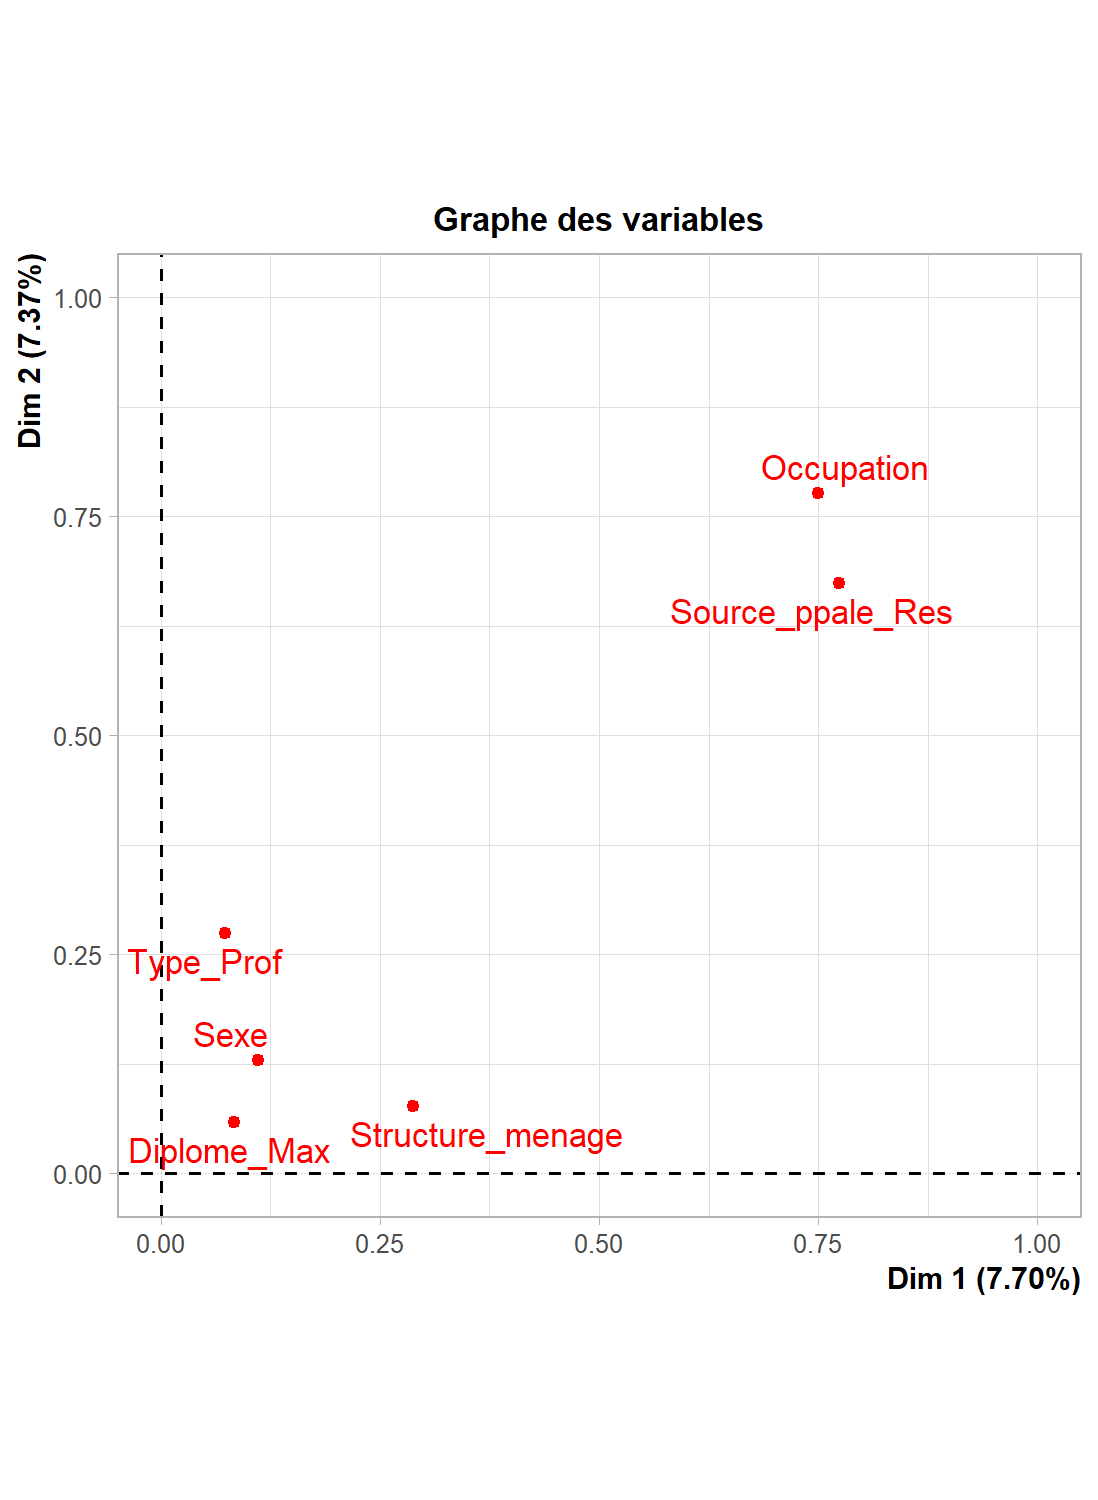
\includegraphics[scale=0.5]{graphiques/MCA1.png}
\caption{Graphique des variables} \label{fig5:MCA1}
\end{figure}
\end{minipage}
\hfill
\begin{minipage}{0.45\textwidth}
\begin{figure}[H]
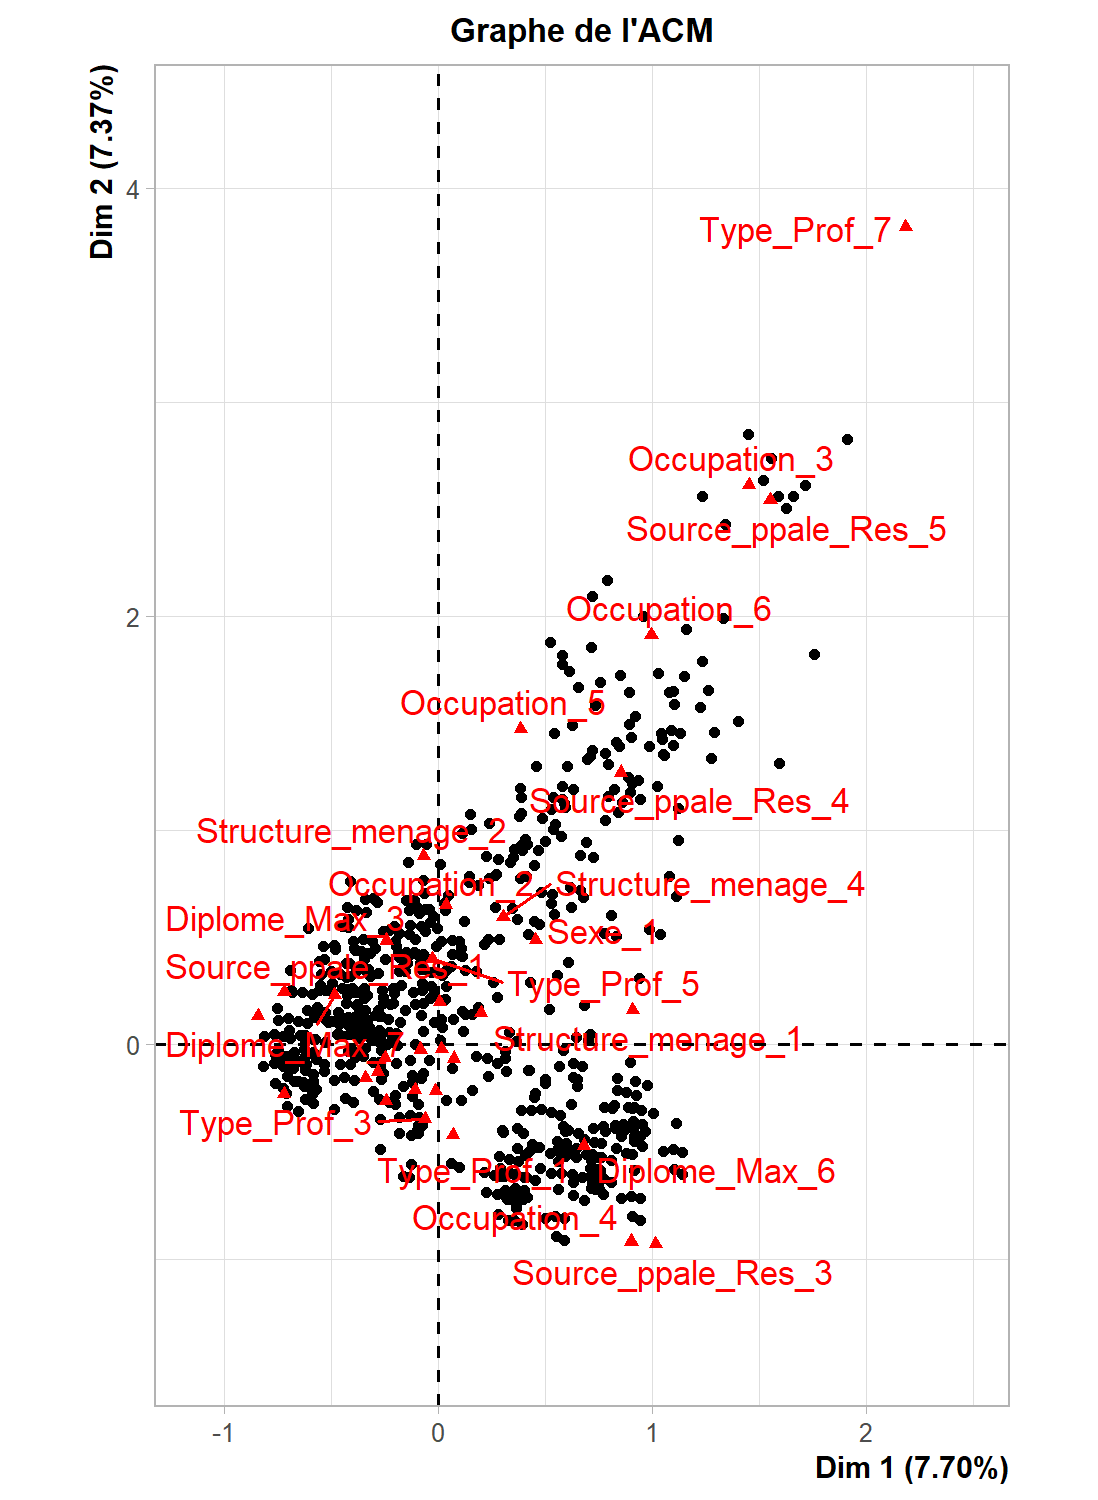
\includegraphics[scale=0.5]{graphiques/MCA2.png}
\caption{Graphiques des modalités des variables / Individus } \label{fig6:MCA2}
\end{figure}
\end{minipage}
\hfill
\end{mdframed}


\subsubsection{Analyse factorielle multiple(AFM)}
Dans le résultat de l'analyse factorielle multiple des ménages, on constate que les coordonnées des groupes de variables qualitatives et quantitatives sont proches sur le premier axe factoriel. Sur l'axe 2 ils ont des groupes très différents sur le second axe factoriel. Cependant lorsqu'on calcul les coefficients Lg et Rv, on constate que les deux groupes de variables pris deux à deux ne sont pas significativement liées. 
\begin{figure}[H]
\centering
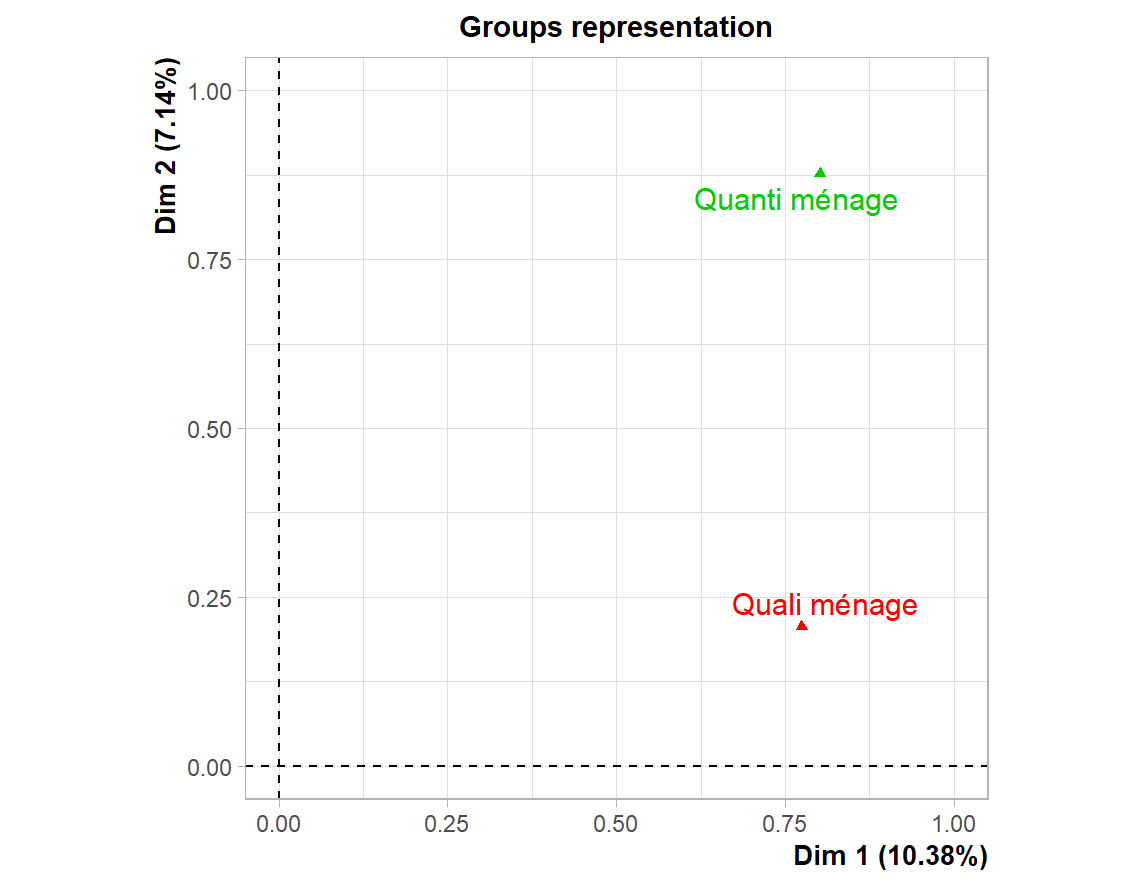
\includegraphics[scale=0.5]{graphiques/AFM_menage.png}
\caption{Graphiques des groupes de l'AFM sur le bloc ménage } \label{fig8:AFM1}
\end{figure}

\subsubsection{AFM sur l'ensemble des variables du jeu de données}
Lorsqu’on analyse les résultats de l’AFM global, on constate que les groupes de variables quali\_logement et quali\_habitude sont proches sur le premier axe factoriel et un peu éloigné sur le second axe. On constate aussi que les groupes de variables du bloc logement (quantitative et qualitative) sont proches à la fois sur le premier axe factoriel et sur le second axe factoriel. 
Globalement, les coefficients Lg et Rv permettent de conclure que les différents blocs de variables ne sont pas significativement liés car les valeurs de ces coefficients sont faibles. Ainsi, nous pouvons conclure à la présence d’une structure par bloc dans notre dataset car ils n’ont pas de lien significatif entre eux.
\begin{figure}[H]
\centering
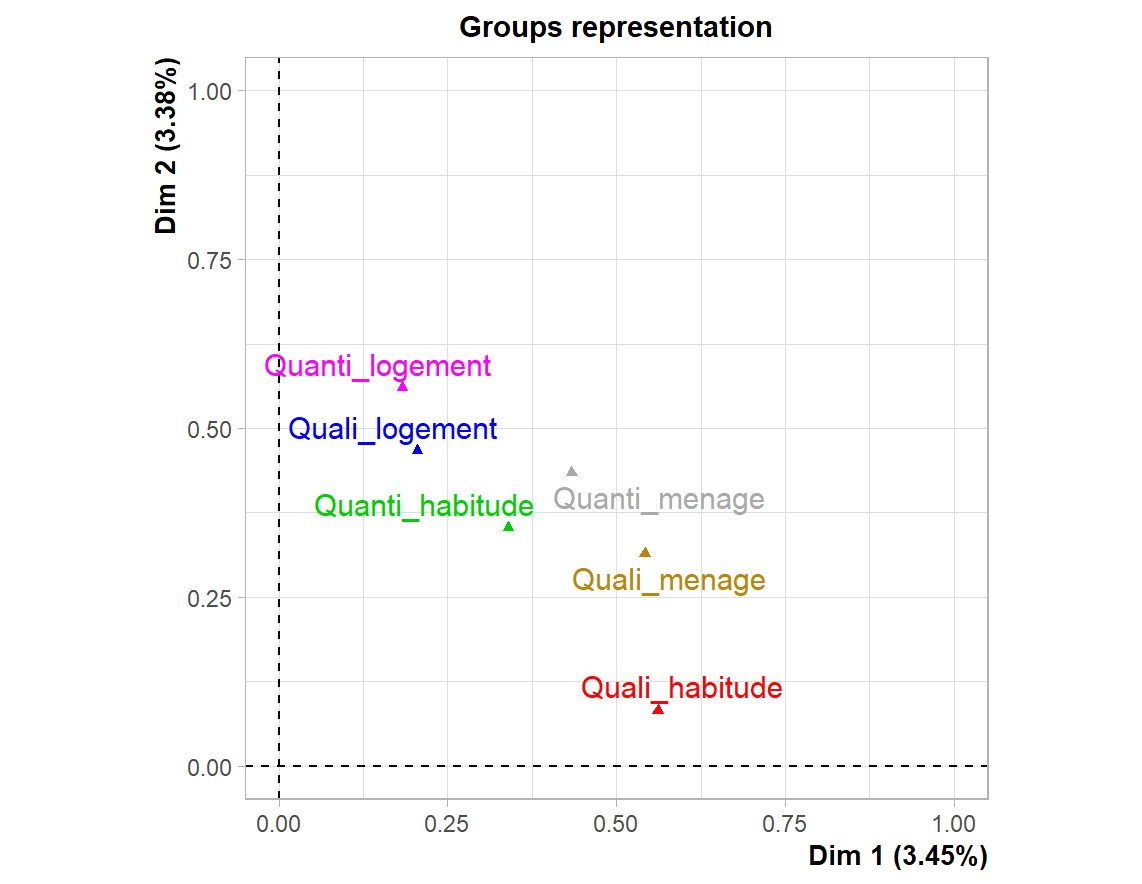
\includegraphics[scale=0.5]{graphiques/AFM_gglobal.png}
\caption{Graphiques des groupes de l'AFM sur l'ensemble des variables } \label{fig9:AFM2}
\end{figure}
\subsubsection{Classification des individus}
Dans cette étape nous souhaitons voir s'il existe une structure en groupe dans les individus (ménages) du jeu de données.  Pour cela nous allons réaliser une classification hiérarchique ascendante sur le jeu de données.
Le but étant de voir s'il existe une structure en groupe au sein des ménages et de calculer les groupes.
Comme nous avons un jeu de données mixtes, nous allons utiliser l'indice de similarité de Gower. L’objectif de cet indice consiste à mesurer dans quelle mesure deux individus sont semblables. L’indice de Gower varie entre 0 et 1. Dans le package cluster, la fonction daisy permet de calculer la distance de Gower définie par : $D_g = 1- S_g$ avec $D_g$ la distance de Gower et $S_g$ l'indice de similarité de Gower. Avec la distance de Gower, deux individus sont identiques si la distance de Gower vaut 0 et ils sont totalement différents si $D_g$ vaut 1.
\begin{figure}[H]
\centering
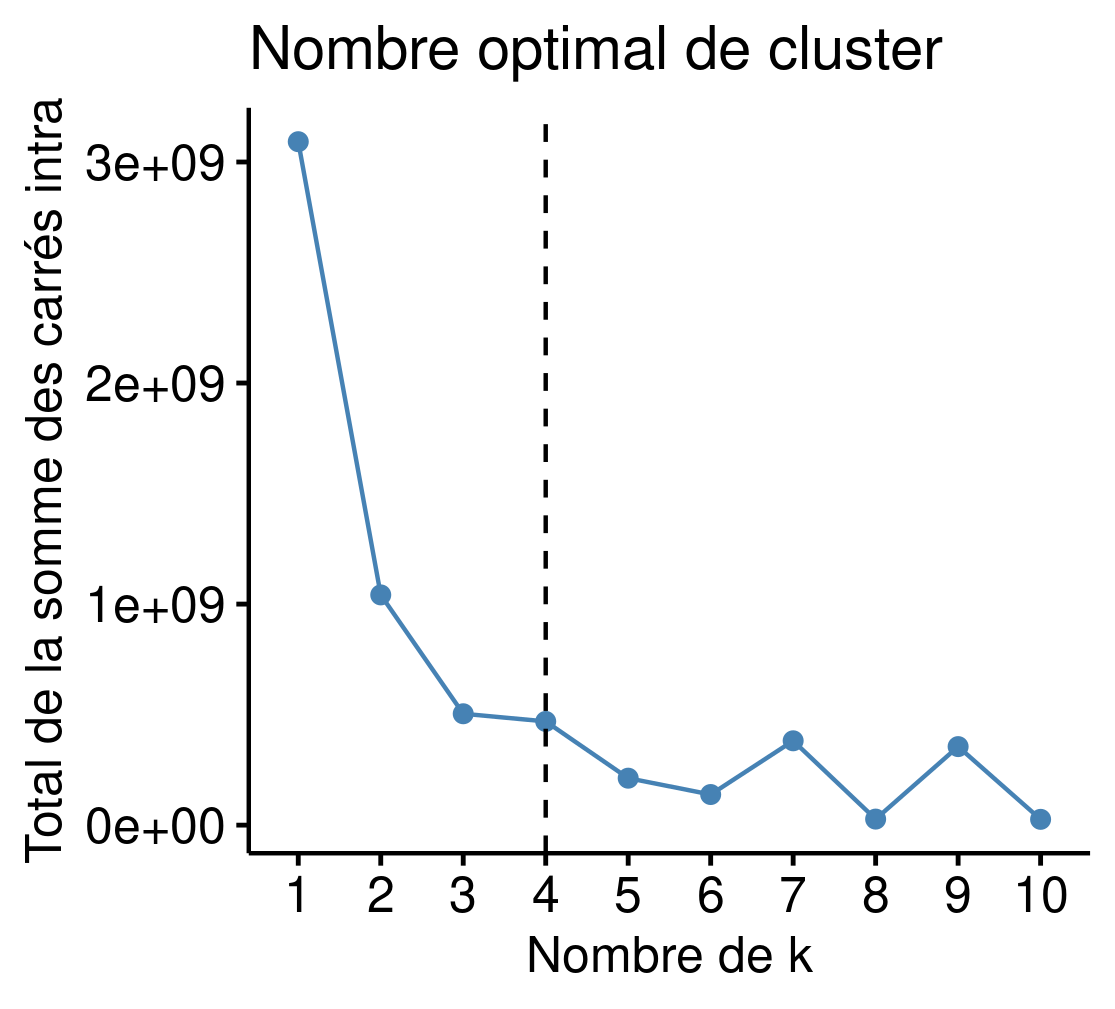
\includegraphics[scale=1]{graphiques/optimal_indiv_clusters.png}
\caption{Graphique résultant de la méthode du coude (Elbow)} \label{fig10:opticlust}
\end{figure}
Le graphique \ref{fig10:opticlust} indique que le nombre optimal de cluster est 4
Nous réalisons un Kmeans sur les résultats de la classification hiérarchique ascendante pour 
consolider les groupes.
\begin{figure}[H]
\centering
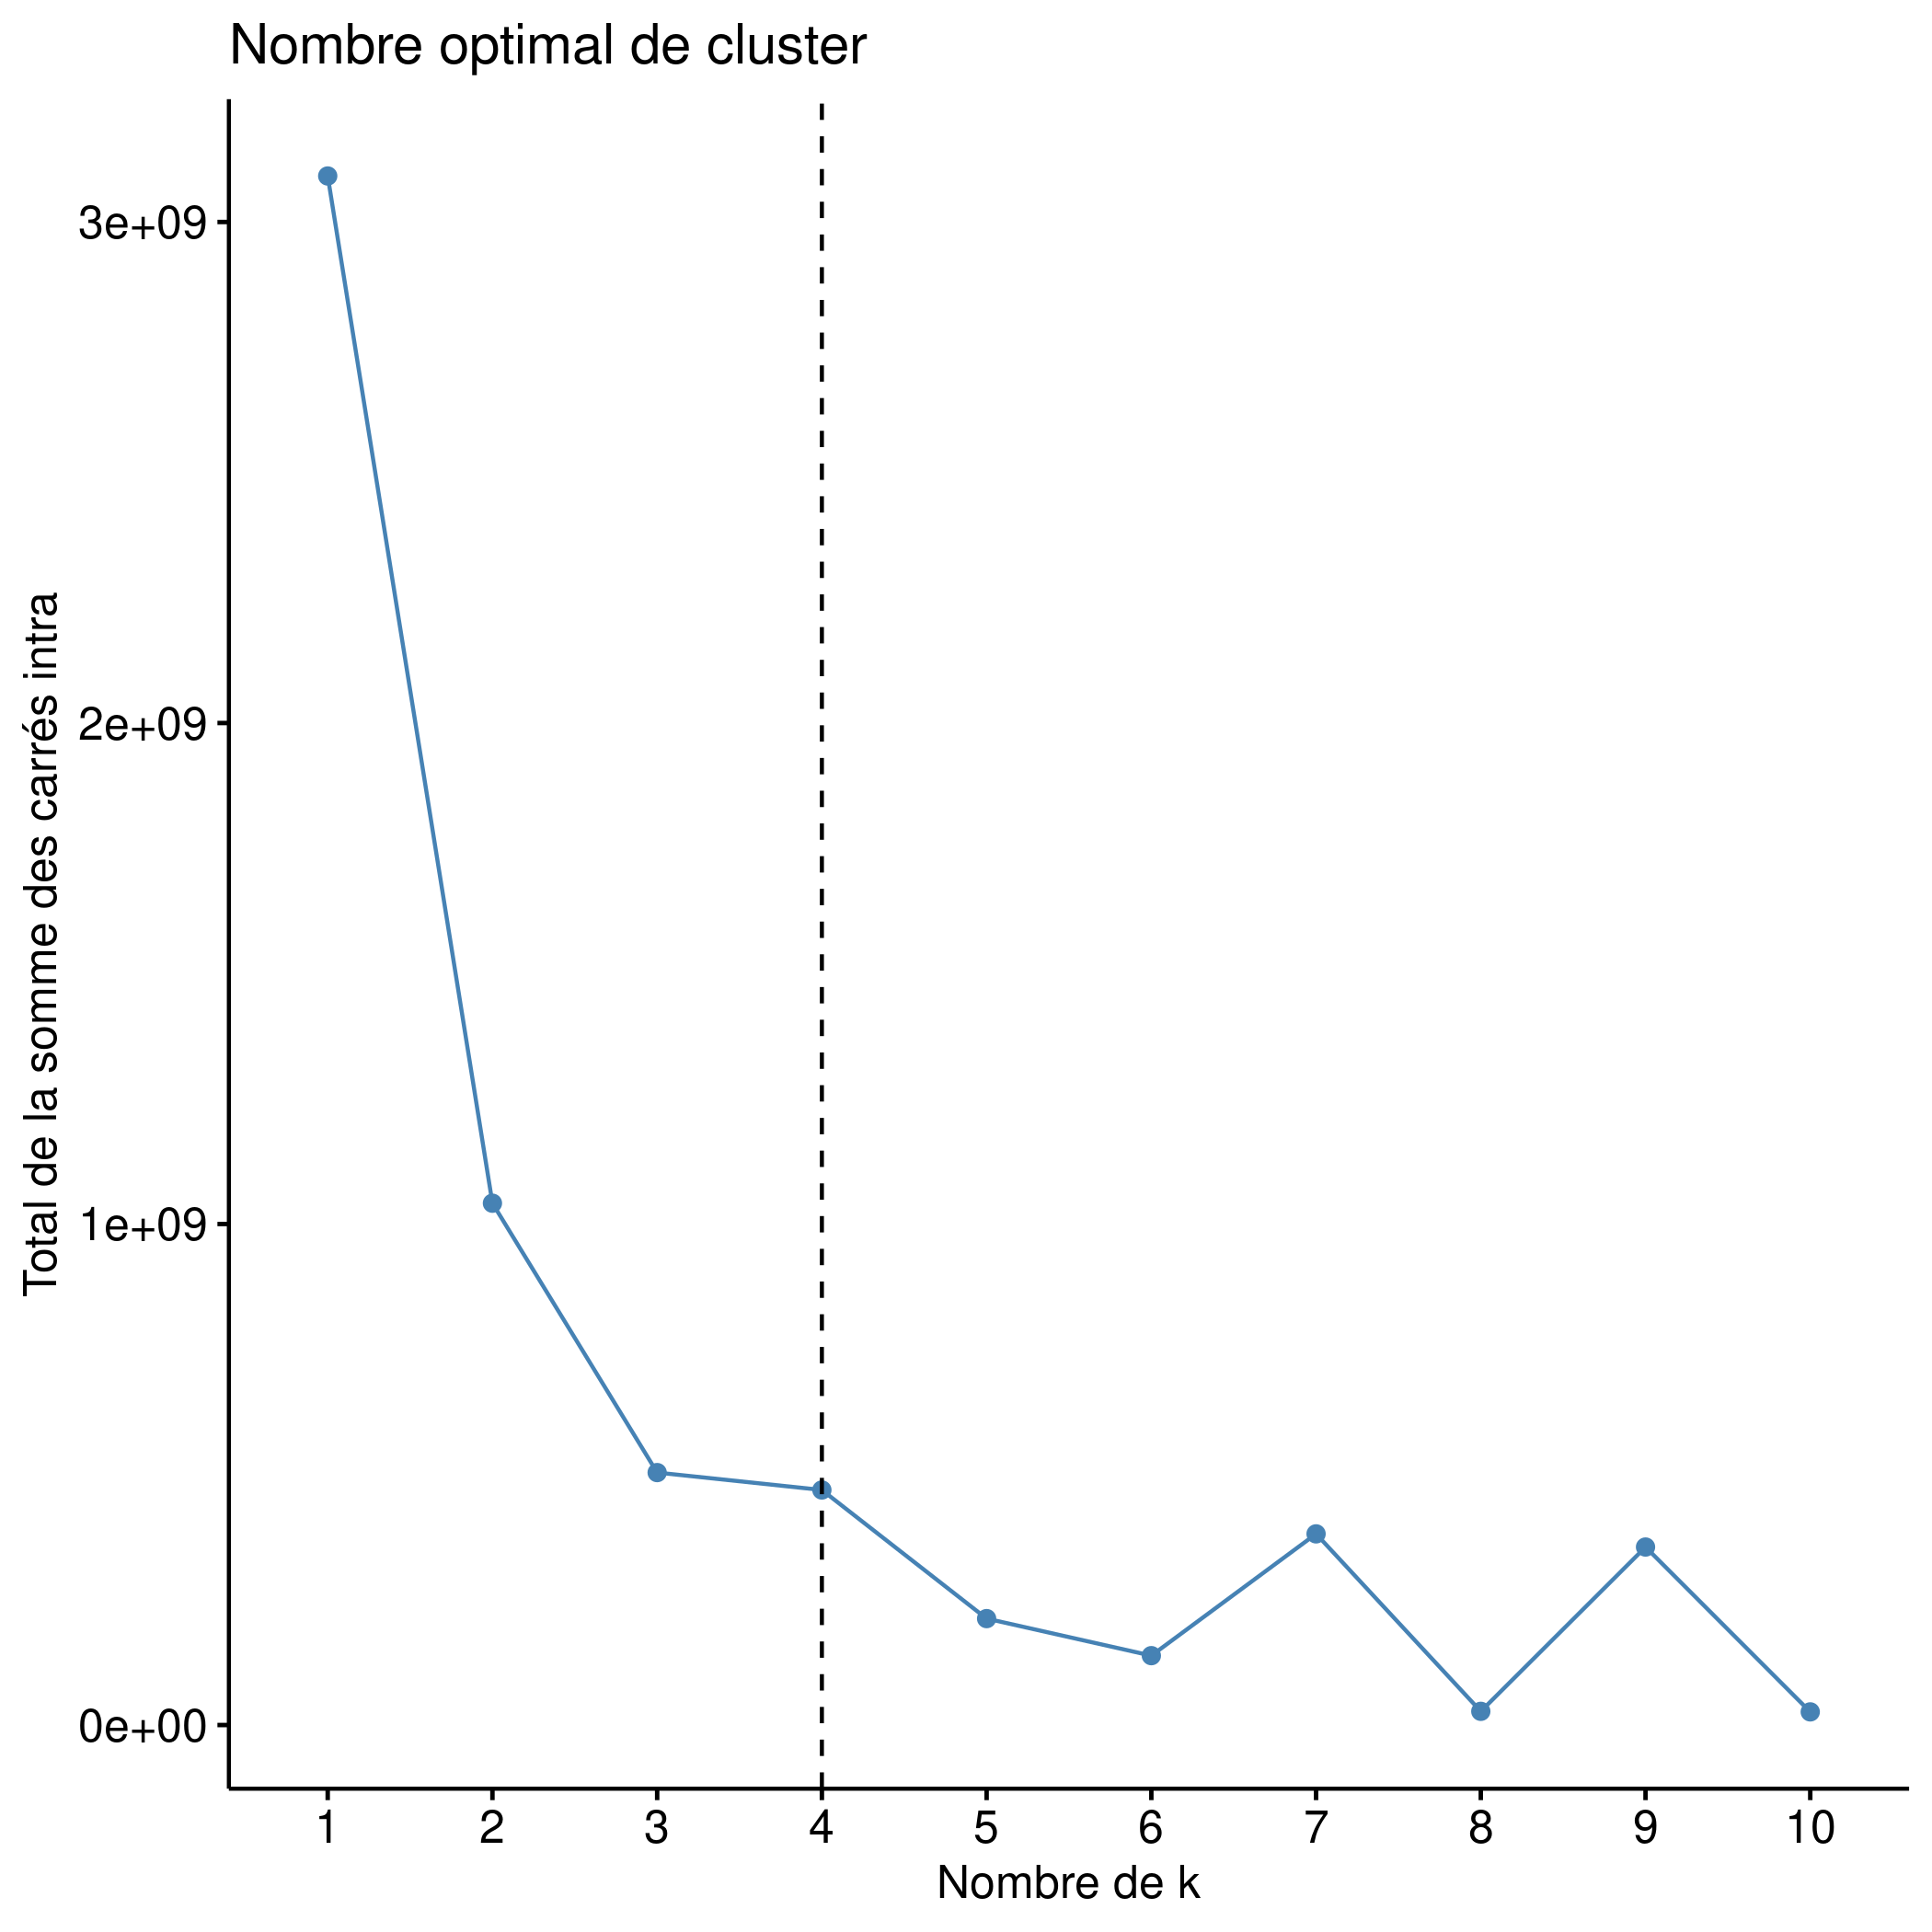
\includegraphics[scale=1]{graphiques/indiv_groups.png}
\caption{Graphique des clusters} \label{fig11:indiv_cluster}
\end{figure}
On observe sur le graphique \ref{fig11:indiv_cluster} 
\subsubsection{Classification des variables}
Le but de la classification de variables est de regrouper ensemble des variables fortement corrélées entre elles en les séparant en classe. Nous utilisons le package ClusterOfVar. La méthode de classification des variables avec ClusterOfVar permet de créer des groupes de variables liées entre elles au sein des groupes et hétérogènes à l’extérieur des groupes. L'avantage principale de cette méthode est qu'elle prend en compte des données mixtes. Le critère d’homogénéité d’une classe est la somme des carrés des corrélations (pour les variables quantitatives) et des rapports de corrélations (pour les variables qualitatives) à une variable synthétique (quantitative) résumant au mieux les variables de la classe. La variable synthétique qui maximise ce critère est la première composante principale de l'AFDM. Deux algorithmes de classifications sont implémentés dans ce package :
\begin{enumerate}
 \item Un algorithme de classification hiérarchique ascendante à travers la fonction hclustvar 
\item Un algorithme itératif de partitionnement
\end{enumerate}
Après avoir implémenté cet algorithme, nous trouvons huit clusters dont 2 sont analysés dans ce rapport.
Cluster 1 :  ce cluster regroupe les variables de structure des ménages, les femmes, les activités ménager (sortie des ordures), les produits de beauté (déodorant, soin visage, …)
Cluster 2 : il rassemble les variables d’habitude des ménages (jardinage, bricolage, séchage de linge dans le logement), l’utilisation d’insecticide, les habitudes de cuisson à l’eau, …

\section{Modélisation et prédiction du Formaldéhyde}
\subsection{Traitement des données manquantes}
Dans le jeu de données la variable cible \textit{Formaldéhyde} présente 3\% de valeurs manquantes.
L'imputation de ces valeurs manquantes est un préalable à l'étape de la modélisation. Nous allons utiliser la méthode d'imputation multiple par chaine de markov MICE(Multiple Imputation by Chained Equations). Cette méthode est basée sur un algorithme Monte-Carlo M
\subsection{Modélisation}
Les différentes méthodes de fouille de données nous ont permis voir que les individus(ménages) ont une structure en groupe donc sont hétérogènes en dehors des groupes. 
Nous avons pu identifier 3 groupes d'individus. Par ailleurs, la classification des variables a permis de mettre en évidence 8 clusters de variables. Cette structure en groupe des individus ne permet pas donc d'appliquer un modèle paramétrique sur l'ensemble du jeu de données. Une alternative pour utiliser des modèles paramétriques serait d'appliquer une modélisation par groupe. L'autre alternative serait d'utiliser des modèles non paramétriques comme les arbres de décisions. Etant donné l'instabilité des résultats des arbres de décisions nous utilisons le choix sera porté sur des modèles d'ensemble de type random forest. L'inconvénient des random forest est que le calcul de l'importance des variables est biaisé lorsque celles-ci sont structurées en blocs et très corrélées au sein des blocs. Ce qui est le cas de notre jeu de données. Une solution pour pallier aux insuffisances des random forest c'est le fuzzy forest. Le fuzzy forest est une extension des random forest et qui permet de calculer l'importance des variables de manière non-biaisée.  
L'algorithme construit une classification de variables. Ensuite il réalise un random forest sur chaque cluster puis selectionne les variables les plus importantes de ses différents modèles pour réaliser un random forest final. L'importance des variables est calculée finalement à partir de ce dernier modèle de random forest.
\subsubsection{Fuzzy forest sur les groupes issues de ClusterOfvar}


\subsubsection{Comparaison et selection de modèle}

\section{Conclusion}


\end{document}

